\documentclass[11pt,a4paper]{article}
\usepackage{ls}
\usepackage[main=english,russian]{babel}

\newcommand{\HGG}[1]{\begin{quote}\textbf{Anmerkung HGG:} #1\end{quote}}

\newenvironment{code}{\tt \begin{tabbing}
\hskip12pt\=\hskip12pt\=\hskip12pt\=\hskip12pt\=\hskip5cm\=\hskip5cm\=\kill}
{\end{tabbing}}
\def\dq{{\char34}}

\title{A Proposal for Modelling TRIZ System Evolution Concepts}

\author{Tom Strempel}

\date{Version of March 9, 2021}

\begin{document}
\maketitle

\section{Aim of the work}

The aim of this paper is to elaborate a proposal for an ontological modelling
of the areas of \emph{TRIZ System Evolution Concepts} based on the approaches
in \cite{TESE2018} and \cite{Shpakovsky2016} and further own investigations.
The work fits into the activities of the \emph{WUMM Ontology Project}
\cite{WUMM} to model core TRIZ concepts using modern semantic web means.  The
work consists of two parts -- a \emph{turtle file}, in which the semantic
modelling is performed based on the SKOS framework \cite{SKOS}, and \emph{this
  elaboration}, in which the backgrounds and motivations of the concrete
modelling decisions are detailed.

\section{Starting point} 

The central concern of practical TRIZ applications is the analysis, evaluation
and transformation of systems in order to improve their operational behaviour.
As in the lecture, the term transformation is understood in a broad sense and
also includes the planning and design of new systems as the transformation of
a system that is only available as vague conceptual requirements into a system
that operates in the real world. TRIZ provides a whole methodological toolbox
that can be used together with domain-specific concepts for the systematic
planning and implementation of such a transformation task. In the seminar we
observed that this TRIZ toolkit is embedded in broader reasoning contexts in
which engineering experience and scientific knowledge are systematised and
generalised.

One of the aspects examined in this context is the evolution of classes of
engineering systems in a historical context in order 
\begin{enumerate}
\item to extract repeating patterns of engineering procedures as «laws»
  \cite{Altshuller1979}, «laws, evolutionary lines and trends» \cite{KS} or
  just «engineering trends» \cite{TESE2018} or
\item to identify evolutionary connections in the unfolding of the history of
  technology \cite{Shpakovsky2016}.
\end{enumerate}

Exploring this aspect, the focus on the exact form of the transformation of a
single system described above was left and, in the style of \emph{distant
  reading}, a variety of information about historical transformations in
different classes of systems has to be analysed in order to extract
transformation patterns from it.  If, for example, the «development of
display» \cite[p. 22]{TESE2018}, \cite[ch. 5]{Shpakovsky2016} is analysed,
this is based on a much stronger abstraction of the system concept compared to
the system concept of classical TRIZ modelling, even if this more
comprehensive abstraction is only rarely explicated in the relevant works --
for example as a \emph{class of systems} in the narrower sense. In the rest of
this paper, the concept of system is used in the same vague generality of an
intuitive understanding as an externally given (metaphysical) concept as in
the referenced works, without attempting to go into more details.

The central to TRIZ understanding, that engineering achievements can be
conceptualised as system transformations, leads in the analysis of historical
technology development to the structure of a directed graph with the
prototypical link
\begin{center}\tt
  OldSystem \textrm{---}\fbox{isTransformedInto}$\to$ NewSystem
\end{center}
In the first approach, this graph is considered as a set of such links to be
classified. The graph structure plays a subordinate role, because even in the
concept of \emph{development line} a rather linear progression is postulated
(e.g. \cite[Figure 4.104]{KS}, but see \cite[4.8.4 and Figure 4.72]{KS}). In
the second approach \cite{Shpakovsky2016}, the graph structure is considered
more consistently, but also with the aim to classify the links in more detail.

The aim of these conceptualisations is on the one hand to develop the
methodology of \emph{evolutionary potential analysis} \cite[4.8.7]{KS} and on
the other hand to consolidate and improve the central TRIZ tools such as the
40 application standards («principles») or the 76 inventive standards.

\section{The Conceptualisations}

The conceptualisations to be developed follow the basic assumptions and
positings that are elaborated in more detail in \cite{Graebe2021}. In
particular, the following namespace prefixes are used:
\begin{itemize}[noitemsep]
\item \texttt{ex:} -- the namespace of a special system to be modelled. 
\item \texttt{tc:} -- the namespace of the TRIZ concepts (RDF subjects).
\item \texttt{od:} -- the namespace of WUMM's own concepts (RDF predicates,
  general concepts). 
\end{itemize}

Our central task is to model the links in concrete evolutionary trees. The
full evolution tree as an edge-marked graph then can be conceptualised as a
set of such links in the usual way.

A link in such a concrete evolution graph has the typical shape
\begin{center}\tt
  ex:TVWithLargePixels ex:decreasePixelSize ex:TVWithMediumPixels .
\end{center}
where the transformation predicate \texttt{ex:decreasePixelSize} is assigned
to certain evolution patterns (even several).
\begin{code}\tt
  ex:decreasePixelSize a rdf:Property, skos:Concept ;\\
  \> od:usesPattern tc:SegmentationPattern ;\\
  \> skos:description {\dq}{\dq}{\dq}Decrease pixel size by segmentation of
  one big pixel\\\>\> in several smaller ones{\dq}{\dq}{\dq}@en. 
\end{code}

\section{Basic concepts}

\subsection{Structured information field}

\begin{enumerate}
    \item Objective classification criteria (objectiveness)
    \item The presence of all significantly different versions (fullness)
    \item Suitable degree of generalisation and specificity
    \item Visualization (to find gaps for patent circumvention)
    \item Sufficient description or prediction of not yet existing versions (informativity)
\end{enumerate}

\subsection{Evolution patterns}
% scope is object, not the technical system

\begin{enumerate}
    \item Mono-Bi-Poly
    \item Trimming
    \item Expanding-trimming
    \item Segmentation
    \item Geometrical evolution
    \item Object structure evolution
    \item Evolution of surface properties
    \item Dynamization
    \item Increasing the controllability
    \item Increasing the coordination of the elements
\end{enumerate}

From these ten basic evolution patterns, more specific evolution patterns can be created. The evolution patterns from one to four are patterns that provide resources for other evolution patterns. For example, it is not possible to dynamize an unsegmented monolith. The structure of the object is given by patterns five to seven. Patterns for dynamization, controllability, and coordination are inserted at points that seem reasonable. This hierarchical structure of transformations is shown in Fig. \ref{fig:basic_evo}.

\begin{figure*}[htb]
	\centering
	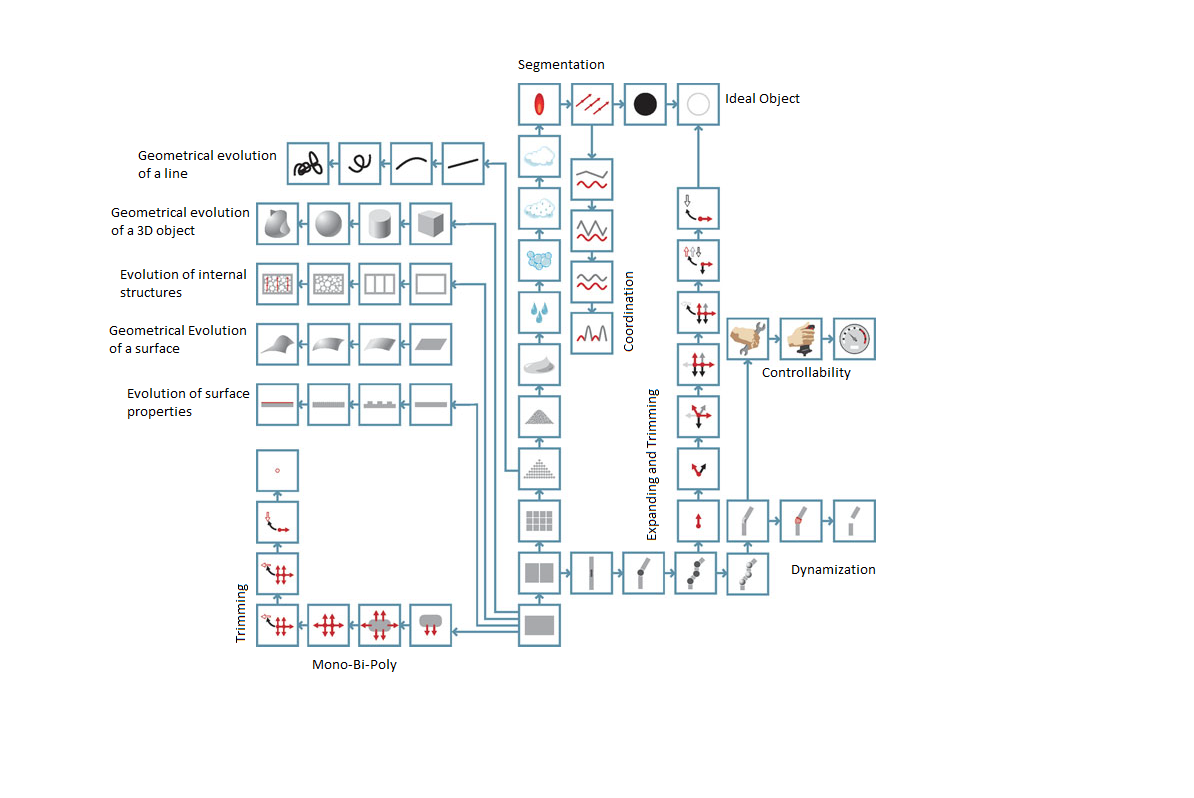
\includegraphics[width=0.99\linewidth]{figures/basictree.png}
	\caption{\small Basic evolution tree \cite{Shpakovsky2016}}
	\label{fig:basic_evo}
\end{figure*}

A transformation is the application of an evolutionary pattern to an object, which subsequently becomes a transformed version of the object.

\subsection{Outside influence}

In the Mono-Bi-Poly pattern the transition to a new mono-system depends on outside influence.

\subsection{Peculiarities about trimming}

\subsection{Evolution trees}

\subsection{Fulfillment of the requirements for a structured information field}

The concepts covered cover all requirements for a structured information field. Objectivity is guaranteed by derivation from a large set of real systems similar to TRIZ. Completeness is guaranteed by using the basic tree for finding all basic versions of an object. For a suitable abstraction btw. specificity a basic or specific evolution tree is used depending on the requirements. Visualizability is guaranteed by the tree structure. Gaps or not completing evolution patterns can be found and described by comparing the basic and specific evolution trees.

\section{Further concepts}

\subsection{Not laws but recommendations}

Shpakovsky never calls his concepts of the evolution pattern and tree laws but uses the terms requirements, rules and, in context with construction instructions, recommendations. Thereby he himself softens the objectivity of his concepts. A really explicit explanation of this change from law to recommendation does not take place, but the circumstance can be understood on the basis of the created evolution tree of the screen.

The trunk of an evolutionary tree, for example, should consist of only one evolutionary pattern (cf. \cite[p. 122f]{Shpakovsky2016}), but it becomes clear that in the case of the screen two evolutionary patterns serve as the trunk, namely trimming and segmenting.
Here it is appropriate, due to the nature of the considered technical system, not to follow the recommendation. This would not be possible with a law or it should not occur at all due to the nature of a law.

\subsection{Determination of not known versions}

\begin{figure*}[htb]
	\centering
	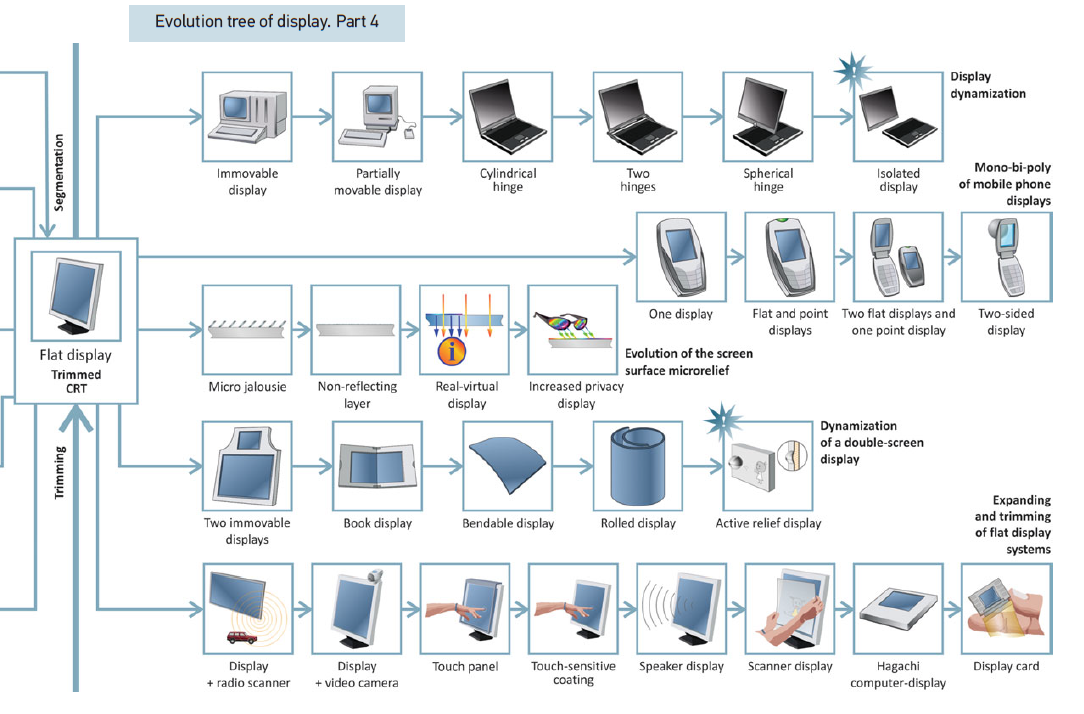
\includegraphics[width=0.9\linewidth]{figures/removable display.PNG}
	\caption{\small Section of the specific evolution tree of the screen \cite{Shpakovsky2016}, see http://www.target-invention.com/ for the complete tree}
	\label{fig:spec_evo}
\end{figure*}


For the analysis of an object, both the basic (see Fig. \ref{fig:basic_evo}) and the specific evolutionary tree (see Fig. \ref{fig:spec_evo}) must be created. By comparing the two trees, gaps as well as unfinished evolutionary patterns can be discovered. The highest level of the pattern of dynamization consists of a complete decoupling of the individual components. For a laptop, this would mean separating the screen and peripherals. At the time the evolutionary tree of the screen was created around 2002, this version of the object did not yet exist. By recognizing this gap, a useful new version was found. Nowadays, complete dynamization is achieved by integrating the computing technology into the screen and connecting the peripherals via Bluetooth. Thus it was shown that evolution trees are able to map future developments.

\subsection{Patent circumvention}

There is often the problem that a patent already exists for a desired product. In this situation it is either possible to pay high license fees to the patent owner or to circumvent the patent.
The legal method of patent circumvention, which consists of using loopholes and erroneous patent descriptions to invalidate a patent, is not always applicable.
It is alternatively possible to modify the object under investigation to develop a better product. This inventive method has the disadvantage of having large development costs and having to change the basic design. On the other hand, it is not possible to obtain an alternative patent without modification.
From this conflict, typical for TRIZ, a synthesis emerges in the form of the legal-inventive method. This new method aims at finding transformation versions not yet covered by patents through evolution trees.
The search for existing patents can be additionally facilitated by using the object and transformation names as keywords.

\section{Modelling}

\subsection{Modelling the evolution tree concepts}

\subsection{Modelling the screen evolution tree}

\subsection{Modelling the ship propulsion evolution tree}

\begin{thebibliography}{xxx}
\raggedright
\bibitem{Altshuller1979} Genrich Altshuller (1979).  Creativity as an exact
  science (in Russian). English version: Gordon and Breach, New York 1988.
\bibitem{Graebe2021} Hans-Gert Gr\"abe (2021). About the WUMM modelling
  concepts of a TRIZ ontology.  \url{https://github.com/wumm-project/Leipzig-Seminar/blob/master/Wintersemester-2020/Seminararbeiten/Anmerkungen.pdf}.
\bibitem{KS} Karl Koltze, Valeri Souchkov (2017).  Systematische
  Innovationsmethoden (in German).  Hanser, Munich. ISBN 978-3-446-45127-8.
\bibitem{TESE2018} Alex Lyubomirsky, Simon Litvin, Sergei Ikovenko et al.
  (2018). Trends of Engineering System Evolution (TESE).  TRIZ Consulting
  Group. ISBN 9783000598463.
\bibitem{Shpakovsky2016} Nikolay Shpakovsky (2016). Tree of Technology
  Evolution. English translation of the Russian original (Forum, Moscow
  2010).\\ \url{https://wumm-project.github.io/TTS.html}
\bibitem{SKOS} SKOS -- The Simple Knowledge Organization System.
  \url{https://www.w3.org/TR/skos-reference/}.  
\bibitem{WUMM} The WUMM Project. \url{https://wumm-project.github.io/} 
\end{thebibliography}

\end{document}
